This appendix describes the steps for installing and running the RAFSINE application on remote \gls{gpu} enabled servers running Ubuntu $16.04$, with the aim of achieving remote visualization of the \gls{opengl} user interface through \gls{vnc} and/or X11-forwarding.

\section{VirtualGL Installation and VNC Configuration}\label{app:virtualgl_install}
First, install the latest NVIDIA drivers. If not using the latest version of Ubuntu, add the \textit{Personal Package Archives} for proprietary NVIDIA drivers\footnote{\url{https://launchpad.net/~graphics-drivers/+archive/ubuntu/ppa}}. At the time of writing, the latest version was 387:\\[\baselineskip]
\shadowbox{%
\begin{minipage}[l]{0.85\textwidth}
\begin{lstlisting}
# add-apt-repository ppa:graphics-drivers
# apt-get update
# apt-get install nvidia-387
\end{lstlisting}
\end{minipage}
}\\[\baselineskip]
Follow any configuration steps required by this installation. Reboot and check that the drivers were loaded:\\[\baselineskip]
\shadowbox{%
\begin{minipage}[l]{0.85\textwidth}
\begin{lstlisting}
$ lsmod | grep nvidia
nvidia_uvm            688128  0
nvidia_drm             49152  2
nvidia_modeset        897024  2 nvidia_drm
nvidia              13971456  79 nvidia_modeset,nvidia_uvm
drm_kms_helper        155648  1 nvidia_drm
drm                   364544  5 drm_kms_helper,nvidia_drm
\end{lstlisting}
\end{minipage}
}\\[\baselineskip]
Optionally, the latest \gls{cuda} can now be installed by following the instructions on the NVIDIA downloads website\footnote{\url{https://developer.nvidia.com/cuda-downloads}}. Check which PCI bus ID is used by the \gls{gpu}:\\[\baselineskip]
\shadowbox{%
\begin{minipage}[l]{0.85\textwidth}
\begin{lstlisting}
$ nvidia-xconfig --query-gpu-info
Number of GPUs: 1

GPU #0:
  Name      : GeForce GTX 1080 Ti
  UUID      : GPU-bfe3f861-3df7-0e3b-6c57-ea4addd8030c
  PCI BusID : PCI:130:0:0

  Number of Display Devices: 0
\end{lstlisting}
\end{minipage}
}\\[\baselineskip]
If using a \gls{gpu} featuring a dedicated general-purpose compute mode, such as the NVIDIA Tesla series, enable graphics rendering by:\\[\baselineskip]
\shadowbox{%
\begin{minipage}[l]{0.85\textwidth}
\begin{lstlisting}
# nvidia-smi --gom=0
GOM changed to "All On" for GPU 0000:03:00.0.
All done.
Reboot required.
\end{lstlisting}
\end{minipage}
}\\[\baselineskip]
\gls{vgl} requires an \gls{x11} server to be running. To this end, install a desktop environment, display manager, and \gls{x11}. Then enable the display manager and set the default runlevel to graphical:\\[\baselineskip]
\shadowbox{%
\begin{minipage}[l]{0.85\textwidth}
\begin{lstlisting}
# apt-get install xfce4 lightdm xorg
# systemctl enable lightdm.service
# systemctl set-default graphical.target
\end{lstlisting}
\end{minipage}
}\\[\baselineskip]
Download and install the latest version of \gls{vgl}\footnote{\url{https://www.virtualgl.org/}} as well as TurboVNC\footnote{\url{https://www.turbovnc.org/}} and install them with:\\[\baselineskip]
\shadowbox{%
\begin{minipage}[l]{0.85\textwidth}
\begin{lstlisting}
# dpkg -i virtualgl_2.5.2_amd64.deb
# dpkg -i turbovnc_2.1.2_amd64.deb
\end{lstlisting}
\end{minipage}
}\\[\baselineskip]
If the display manager is running, stop it before configuring \gls{vgl}. Follow the instructions in the configuration script:\\[\baselineskip]
\shadowbox{%
\begin{minipage}[l]{0.85\textwidth}
\begin{lstlisting}
# systemctl stop lightdm.service
# vglserver_config
\end{lstlisting}
\end{minipage}
}\\[\baselineskip]
Next, configure \gls{x11} to not use the \gls{gpu} as a display device, and supply the PCI bus ID from before:\\[\baselineskip]
\shadowbox{%
\begin{minipage}[l]{0.85\textwidth}
\begin{lstlisting}
# nvidia-xconfig --use-display-device=none --busid="PCI:130:0:0"
\end{lstlisting}
\end{minipage}
}\\[\baselineskip]
Reboot, and check that everything is working:\\[\baselineskip]
\shadowbox{%
\begin{minipage}[l]{0.85\textwidth}
\begin{lstlisting}
$ ps aux | grep Xorg | grep -v grep
root  2498  0.3  0.0 170224 48784 tty7  Ss+  08:23  1:25 
    /usr/lib/xorg/Xorg -core :0 -seat seat0 -auth 
    /var/run/lightdm/root/:0 -nolisten tcp vt7 -novtswitch
$ systemctl status lightdm.service
    lightdm.service - Light Display Manager
    Loaded: loaded (/lib/systemd/system/lightdm.service; 
    enabled; vendor preset: enabled)
    Active: active (running) ...
\end{lstlisting}
\end{minipage}
}\\[\baselineskip]
Start the \gls{vnc} server:\\[\baselineskip]
\shadowbox{%
\begin{minipage}[l]{0.85\textwidth}
\begin{lstlisting}
$ vncserver -geometry 1920x1200 -3dwm
\end{lstlisting}
\end{minipage}
}\\[\baselineskip]
Connect to the first screen of the \gls{vnc} server using e.g. \texttt{109.225.89.135:1}. This should start the desktop environment (Xfce4 in this case). To check that \gls{vgl} is working, try running the \gls{opengl} example application \texttt{glxgears}. Since the \gls{vnc} server was started with the \texttt{-3dwm} option, \gls{opengl} applications can be started normally by for example typing their name in a terminal. Without this option, the application name has to be prepended with \texttt{vglrun} to indicate 3D support is required. The environment variable \texttt{VGL\_LOGO=}1 displays the \gls{vgl} logo:\\[\baselineskip]
\shadowbox{%
\begin{minipage}[l]{0.85\textwidth}
\begin{lstlisting}
# apt-get install mesa-utils
$ VGL_LOGO=1 vglrun glxgears
\end{lstlisting}
\end{minipage}
}\\[\baselineskip]
The result should look like figure~\ref{fig:virtualgl_glxgears}.
\begin{figure}[ht]
\begin{center}
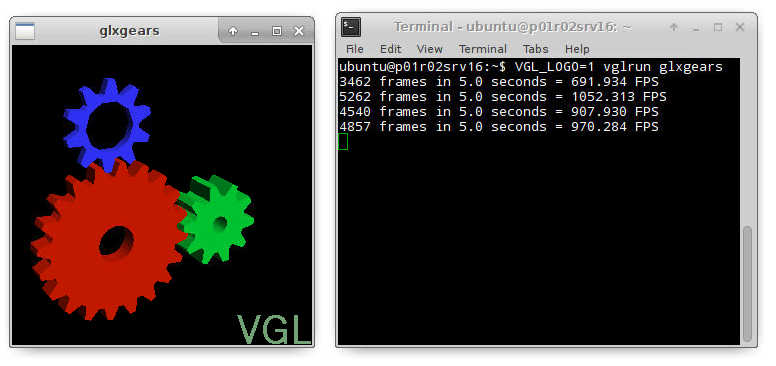
\includegraphics[width=1.0\linewidth]{virtualgl_glxgears.jpg}
\end{center}
\caption{The \gls{opengl} example application \texttt{glxgears} using hardware accelerated 3D rendering through \gls{vgl} over \gls{vnc}.}
\label{fig:virtualgl_glxgears}
\end{figure}
When executing the program through a debugger such as \gls{gdb}, \gls{vgl} can be loaded indirectly by setting an environment variable inside \gls{gdb}:\\[\baselineskip]
\shadowbox{%
\begin{minipage}[l]{0.85\textwidth}
\begin{lstlisting}
set environment LD_PRELOAD=/usr/lib/libvglfaker.so
\end{lstlisting}
\end{minipage}
}\\[\baselineskip]
Since the \gls{vnc} server is only protected by a password as default, it can be a potential security hazard. This can be mitigated by only allowing local connections to the \gls{vnc} server, tunneled from a client by \gls{ssh}. Start the remote \gls{vnc} server with\\[\baselineskip]
\shadowbox{%
\begin{minipage}[l]{0.85\textwidth}
\begin{lstlisting}
$ vncserver -geometry 1920x1200 -localhost -3dwm
\end{lstlisting}
\end{minipage}
}\\[\baselineskip]
and an \gls{ssh}-tunnel on the client by:\\[\baselineskip]
\shadowbox{%
\begin{minipage}[l]{0.85\textwidth}
\begin{lstlisting}
$ ssh username@$REMOTE_IP -x -e none 
	-L $LOCAL_VNC_PORT:127.0.0.1:$REMOTE_VNC_PORT
	-p $REMOTE_SSH_PORT
\end{lstlisting}
\end{minipage}
}\\[\baselineskip]
for example \\[\baselineskip]
\shadowbox{%
\begin{minipage}[l]{0.85\textwidth}
\begin{lstlisting}
$ ssh ubuntu@109.225.89.135 -x -e none 
	-L 5901:127.0.0.1:5901 -p 31761
\end{lstlisting}
\end{minipage}
}\\[\baselineskip]
The \texttt{-x} switch disables X11-forwarding, while \texttt{-e none} disables escape characters, neither of which is useful when connecting through VNC. Now the client can connect to \texttt{localhost:1} in a \gls{vnc} viewer. All \gls{vnc} network traffic between client and server will be encrypted, and the only way to access the \gls{vnc} server is by connecting and tunneling through \gls{ssh}. Using the TurboVNC client is advisable since it was developed by the VirtualGL team for this purpose.

\section{VirtualGL through SSH X11-forwarding}
VirtualGL can also be made to work through SSH X11-forwarding, as long as the client is running an X11-server. This solution has the advantage of seamless integration with the X11 window manager on the client, and slightly less \gls{cpu} usage on the server side. Follow the steps in chapter \ref{app:virtualgl_install} to install and configure \gls{vgl}.

On Ubuntu, X11-forwarding is enabled on the \gls{ssh} server by default. Check that normal X11-forwarding is working by connecting with the \texttt{-X} option\\[\baselineskip]
\shadowbox{%
\begin{minipage}[l]{0.85\textwidth}
\begin{lstlisting}
$ ssh username@$REMOTE_IP -X -e none -p $REMOTE_SSH_PORT 
\end{lstlisting}
\end{minipage}
}\\[\baselineskip]
and running a non-\gls{opengl} application such as \texttt{xclock}. If the forwarding works, exit the \gls{ssh} connection, and reconnect to the server with\\[\baselineskip]
\shadowbox{%
\begin{minipage}[l]{0.85\textwidth}
\begin{lstlisting}
$ vglconnect -s username@REMOTE_IP -e none -p $REMOTE_SSH_PORT
\end{lstlisting}
\end{minipage}
}\\[\baselineskip]
This will automatically open a network stream called \textit{VGL Transport} which is essentially a dedicated TCP socket for sending encoded or compressed 3D images between client and server. \gls{opengl} applications can then be launched from the terminal by typing their name prepended with \texttt{vglrun}.
\clearpage
\section{Installing the RAFSINE Dependencies}\label{app:rafsine_deps}
Install the latest NVIDIA \gls{gpu} drivers as described in appendix~\ref{app:virtualgl_install}, then the latest \gls{cuda} toolkit by following the instructions on the NVIDIA downloads website\footnote{\url{https://developer.nvidia.com/cuda-downloads}}.

The rest of the build dependencies can be installed by the package manager,\\[\baselineskip]
\shadowbox{%
\begin{minipage}[l]{0.85\textwidth}
\begin{lstlisting}
# apt-get install libboost-all-dev lua5.1 pkg-config \
	libglew-dev freeglut3-dev libjpeg9-dev \
	libpthread-stubs0-dev libc6-dev gcc-6-base luarocks \
	libfltk1.3-dev libglfw3-dev \
	cmake
\end{lstlisting}
\end{minipage}
}\\[\baselineskip]
and by \texttt{luarocks}\\[\baselineskip]
\shadowbox{%
\begin{minipage}[l]{0.85\textwidth}
\begin{lstlisting}
# luarocks install penlight
# luarocks install multikey
\end{lstlisting}
\end{minipage}
}\\[\baselineskip]


